\lstdefinestyle{DOS}
{
    backgroundcolor=\color{white},
    basicstyle=\scriptsize\color{black}\ttfamily
}
\vspace{10mm}
\section{Step Response of the da Vinci Robot in 3D Cartesian Space}\label{sec:step_3d}
This test is carried out in a similar manner as the test in \autoref{app:meas_1}, now subscribing to the full \texttt{joint\_state} topic (\texttt{rostopic echo joint\_states}) as described in \autoref{app:meas_1}. This displays the measurements of the joint angles from the potentiometers, that correspond to angles in radians (and for \texttt{instrument\_slide}: in meters), secured by the calibration of the motor gearings. An example of a measurement can be seen in \autoref{app:meas_1}.

The measurements are copied directly from the terminal output, and the joint measurements extracted from this string. Use the MATLAB script and the recorded measurement data found in \autoref{app:cd} under the path \texttt{matlab\_scripts/step\_3d/3d\_time\_const\_measurement.m}, to plot the recorded step responses. The step responses for steps in the $x$, $y$ and $z$ direction are shown in \autoref{fig:stepresponses_3d}.

\begin{figure}[h]
\hspace{-16mm}
\subbottom{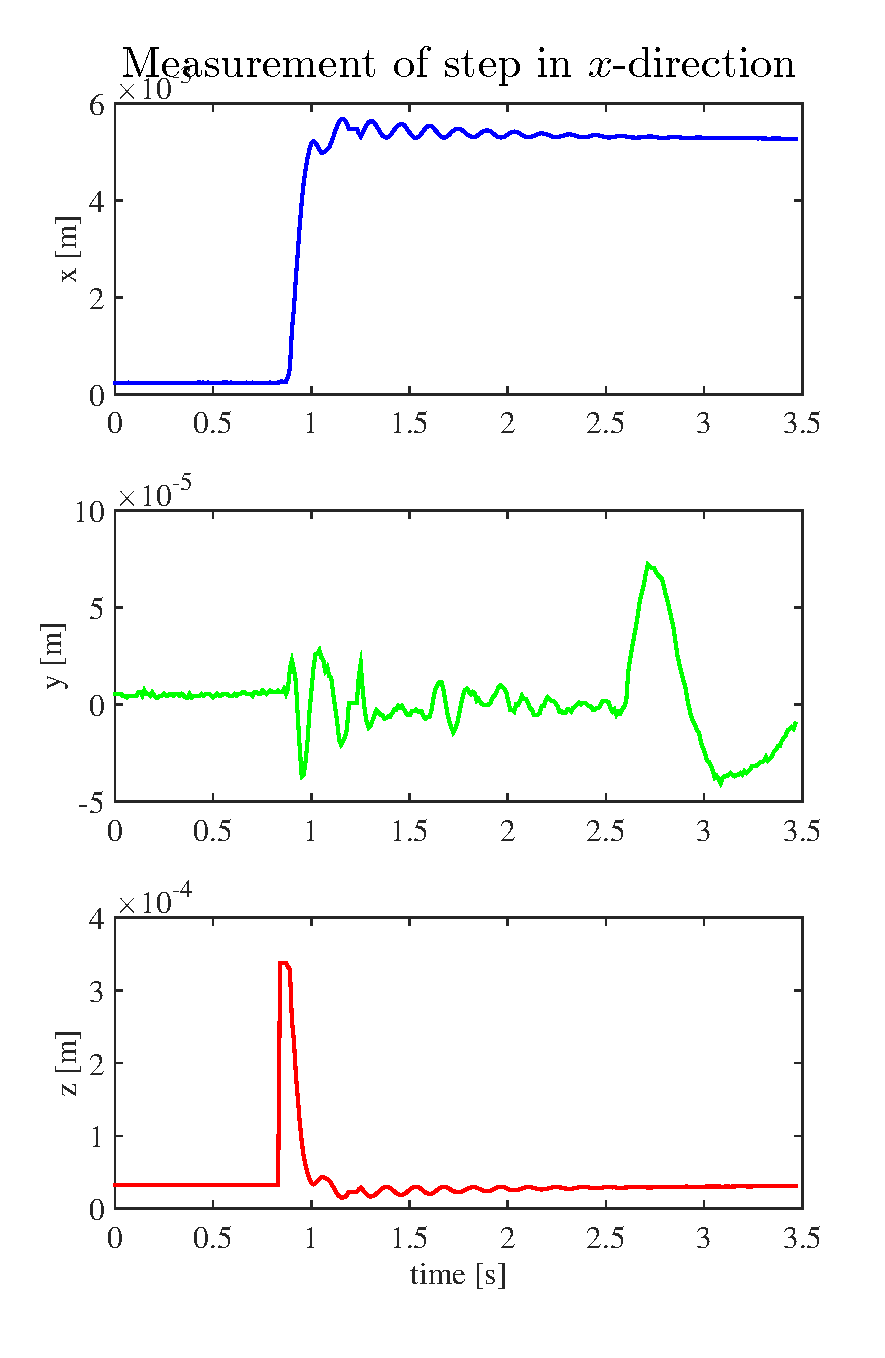
\includegraphics[width=0.4\textwidth]{3d_step_x_5mm.pdf}}%
\subbottom{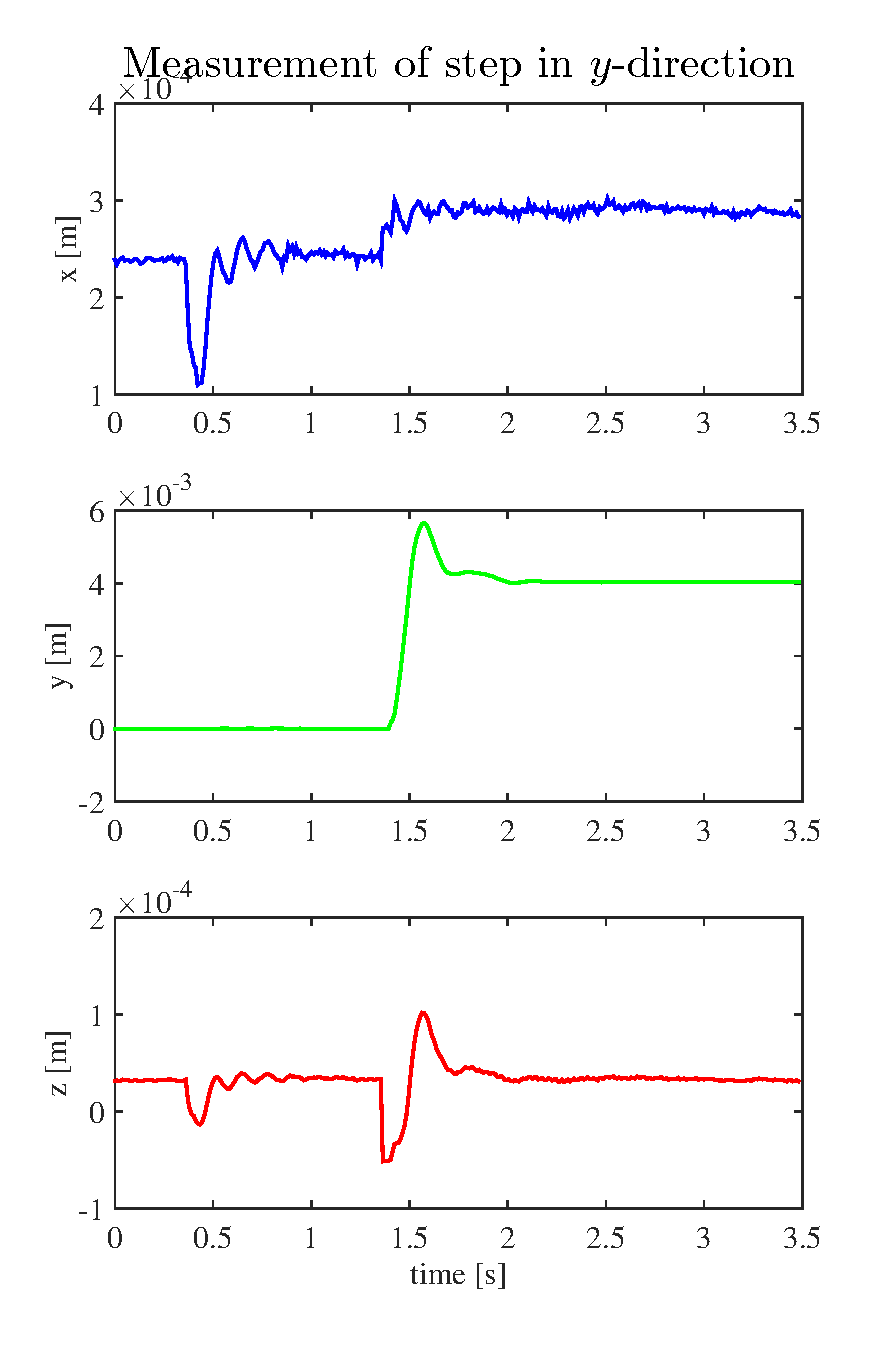
\includegraphics[width=0.4\textwidth]{3d_step_y_5mm.pdf}}%
\subbottom{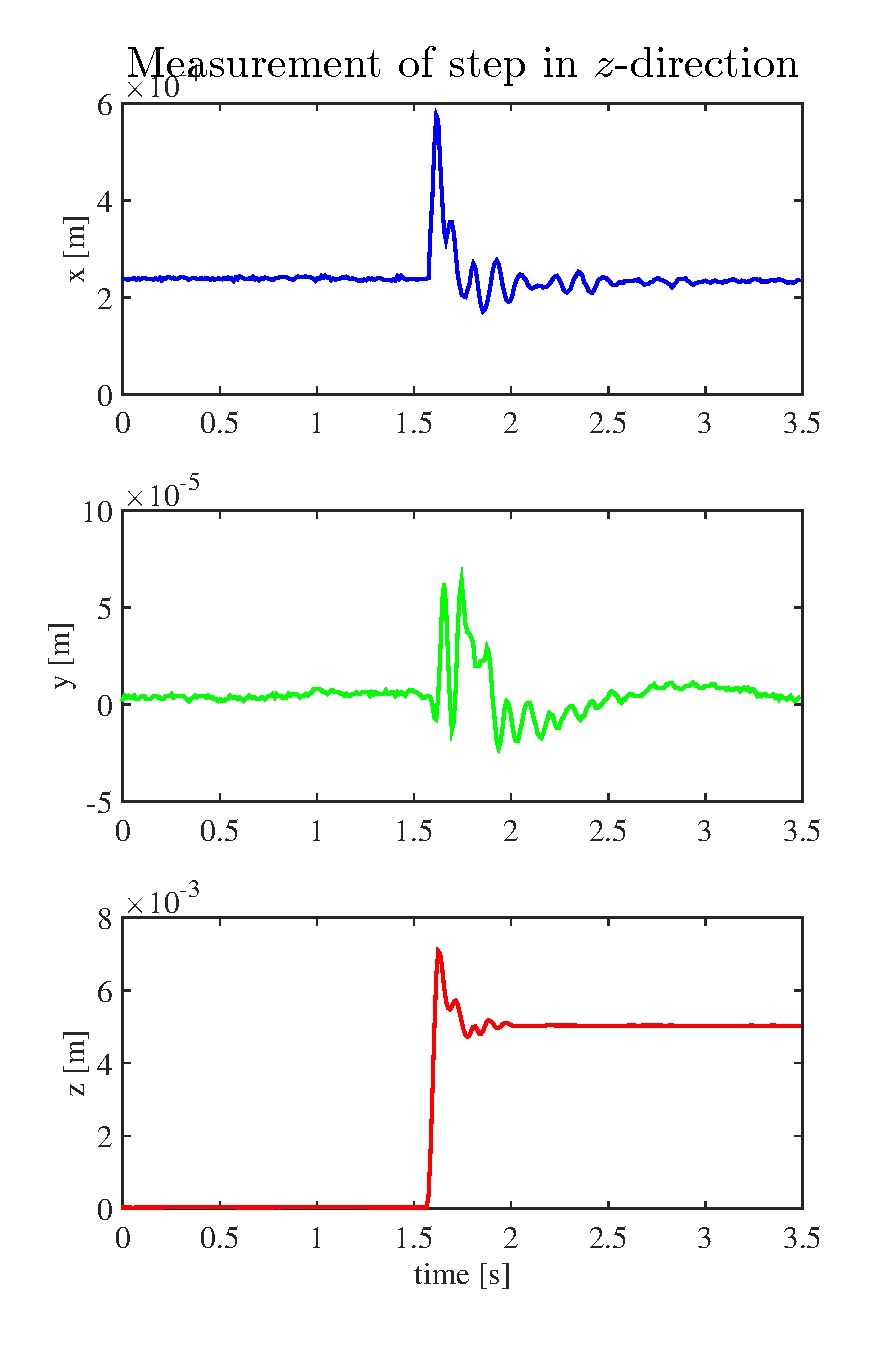
\includegraphics[width=0.4\textwidth]{3d_step_z_5mm.pdf}}%
\caption{Step responses for the $x$, $y$ and $z$ directions from 0\,mm to 5\,mm. Plot details and measurements can be found in \autoref{app:cd} in \texttt{matlab\_scripts/step\_3d/3d\_time\_const\_ measurement.m}}. 
\label{fig:stepresponses_3d}
\end{figure}

\vspace{-0.3cm}
From the plots it is seen, as expected, that a step in one Cartesian coordinate direction is not completely decoupled from the other two directions, because of the movements being implemented by the six revolute joints of the da Vinci robot. It is, on the other hand, also seen that the movements in the other directions are sub-millimeter and that they settle approximately at their initial value. Thus it is considered that the three directions can be seen as approximately decoupled, and a first order approximation of the step response for each direction is presented in \autoref{fig:stepresponses_xyz}.

\begin{figure}[h]
	\centering
	\subbottom{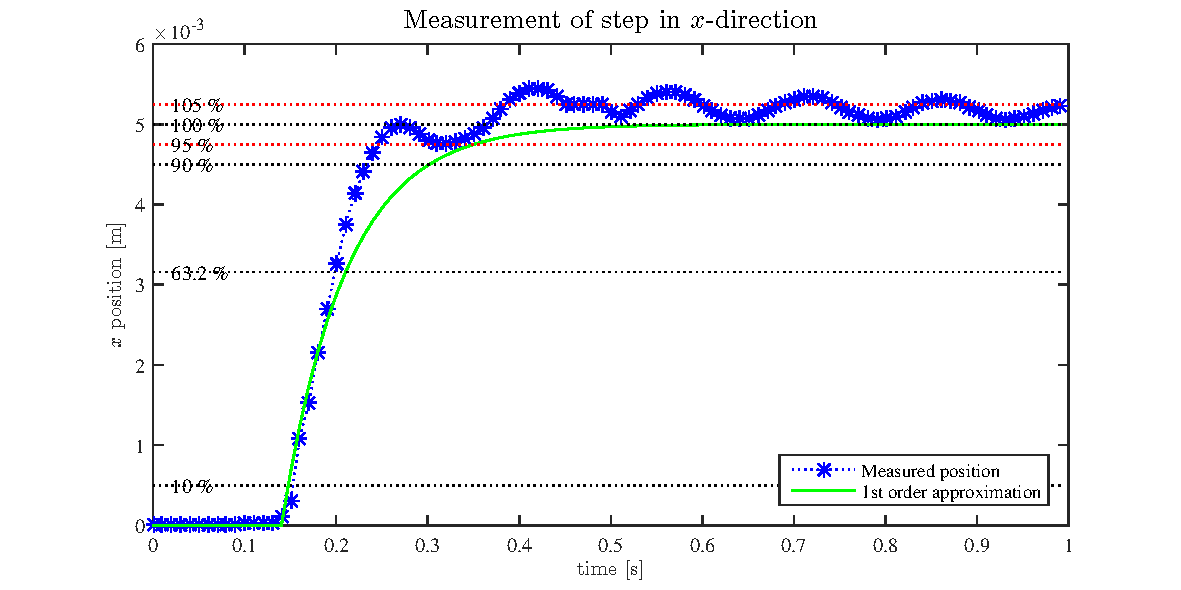
\includegraphics[width=0.9\textwidth]{3d_step_x_approx.pdf}}%
	\hspace{1mm}
	\subbottom{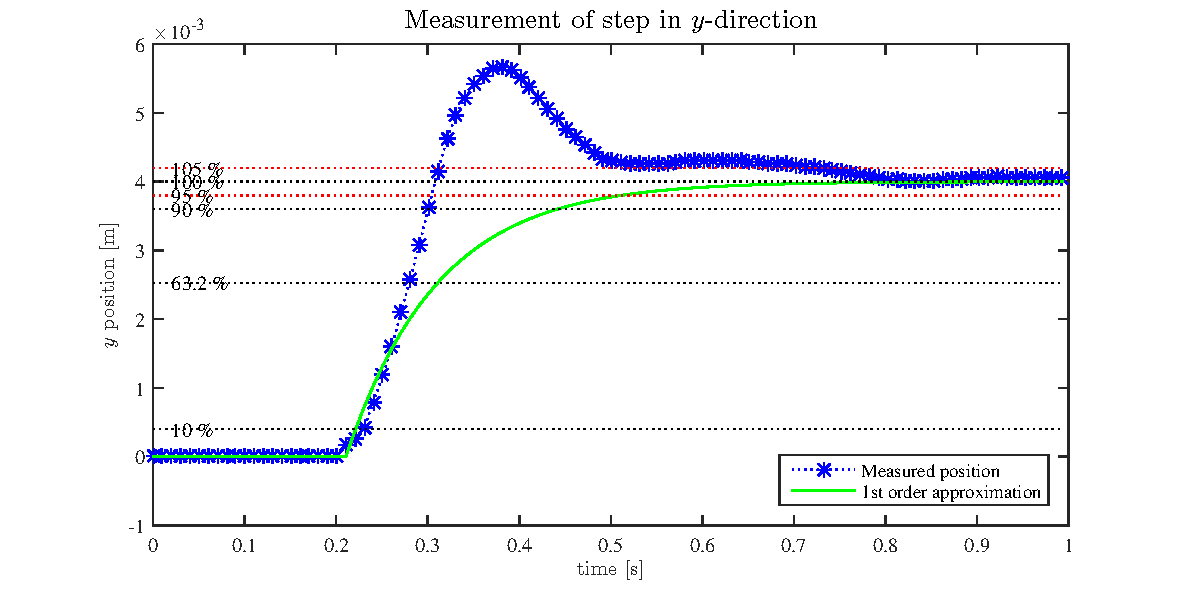
\includegraphics[width=0.9\textwidth]{3d_step_y_approx.pdf}}%
	\hspace{1mm}
	\subbottom{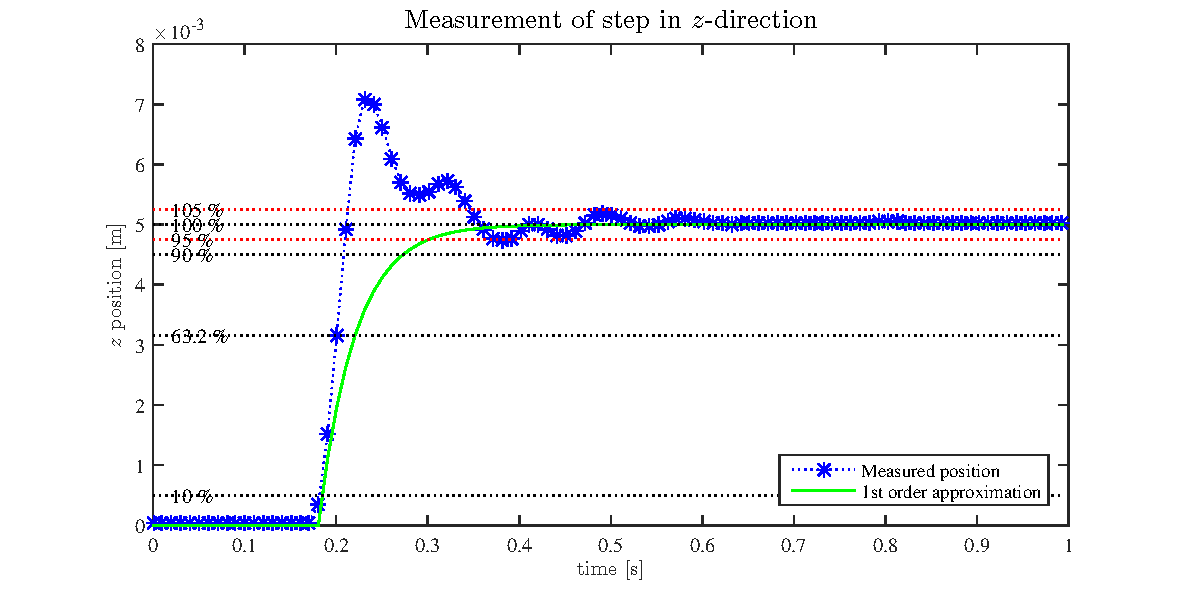
\includegraphics[width=0.9\textwidth]{3d_step_z_approx.pdf}}%
	\caption{Step response for each direction  from 0\,mm to 5\,mm along with first order approximations. It is seen how uncertainties in the $y$ direction cause the robot to step to only 4\,mm. Plot details and measurements can be found in \autoref{app:cd} in \texttt{matlab\_scripts/ step\_3d/3d\_time\_const\_measurement.m}}. 
	\label{fig:stepresponses_xyz}
\end{figure}

For the step in the $x$ direction it is seen how the end effector oscillates for a long time after the step movement, which can be attributed to the flexibility of the structure. The step in the $x$ direction is mainly implemented through a \texttt{hand\_pitch} angle change (see \autoref{fig:naming_convention}).

It is seen how the step input of 5\,mm in the $y$ direction only causes a robot movement of 4\,mm in this direction. This is experiences in all tests, and is attributed to uncertainties in the kinematics and in the inverse kinematics solver. The step in the $y$ direction is mainly implemented through a \texttt{hand\_roll} angle change (see \autoref{fig:naming_convention}).

The step in the $z$ direction is mainly implemented through a \texttt{instrument\_slide} angle change (see \autoref{fig:naming_convention}), and should be comparable to \autoref{fig:stepresponseslideapp}. It is, however, seen that the dynamics have changed, which is expected since an inverse kinematics solver is employed (see \autoref{britt}). This does not explain the considerably lower time constant, which may be explained by a change in the ROS setup from using MoveGroup for publishing control signals to doing it directly (see \autoref{app:ros} for an overview of the two approaches to publishing control signals in ROS), or from changes in the low level controllers and joint motor gearings.




The time constants inferred from these measurements are
\begin{align*}
\tau_x &= 70.088 \text{ ms}\\
\tau_y &= 100.288 \text{ ms}\\
\tau_z &= 40.114 \text{ ms}
\end{align*}

